\chapter{Introduction}
\label{sec:intro}
Fluorescence microscopy is an old technique that has been established
in live sciences for a long time. Being able to see things happening
at the micrometre scale is the fundamental path to understand life and
disease.

Innovation continuously improves microscopy and occasionally new
fields of research are opened up: The discovery and development of
fluorescent proteins initiated a revolution in how microscopy can be
applied in living specimen. 

Optical high resolution techniques allow to observe biological
processes at the scale of individual molecules (tens of nm).

Labels that report membrane potentials or viscosity within cells,
compounds that locally release chemicals when illuminated by light or
even ion pumps that can be switched by light promise novel interesting
research.

All these techniques have in common, that excitation light has to
reach a focal point, line or plane within the sample. For this the
light has to traverse a more or less dense distribution of
fluorophores.  With few exceptions (2-photon, SPIM) microscopes are
generally not optimized for exciting only the in focus fluorophores.

\figref{fig:celegans-devel} compares time lapse experiments on three
different \emph{Caenorhabditis elegans} embryos with varying
illumination intensities. These are small invertebrates. The adult
form is approximately \unit[1]{mm} long . Their anatomy and normal
development are comparatively simple and have been well characterized
\citep{Durbin1987}.

The lineage tree of two developing \emph{C. elegans} embryos is the
same.  Even the number of somatic cells is constant in the organism
(959). With all other factors being equal, particularly the
temperature constant at room temperature, two different embryos will
develop at the same speed from egg to fertile adult in three and a
half days. This makes the following experiment possible, which has
been conducted by Jean-Yves Tinevez at Institut Pasteur.

Embryos are removed from their mothers at an identical stage, before
any cellular divisions have occured. A $z-$stack of the egg with 41
slices and $\unit[1]{\mu m}$ $z-$sampling is obtained every 2 minutes
of the egg.

Each column in \figref{fig:celegans-devel} shows an embryo at the
beginning, after one hour and after two hours and 38 minutes of
development. The left embryo was illuminated with only 0.5\% of the
maximum illumination intensity possible (controlled by AOTF). The
middle embryo was illuminated with 5\% and for the right embryo an
excitation power of 20\% was used.

The images show maximum intensity projections of the $z-$stacks and
each image was normalized so that its darkest pixel is black and its
brightest pixel is white. Comparing the images in the top row from the
start of the development the left image\footnote{Note, that the left
  image in \figref{fig:celegans-devel} is the noisiest in the top
  row. This is due to the photon shot noise, which is Poisson
  distributed.} contains the least amount of fluorescence photons and
the right image the most.

One hour into the experiment, we observe that the right embryo with
the highest excitation dosage died and its fluorophores were bleached.
Some cells even turned apoptotic and went into programmed cell death.

After two hours and 38 minutes the left embryo, that received the
lowest dosage, has developed the most cells. The middle embryo ceased
developing. Reactive oxygen species created by Cells in presence of
reactive oxygen species under oxidative stress activate a DNA damage
checkpoint and arrest their cell cycle progression so as to allow for
repair and prevention of the transmission of damaged or incompletely
replicated chromosomes. The right embryo died much earlier and nearly
all its fluorophores are bleached at the end of the experiment.

% Molecular mechanisms of mammalian DNA repair and the DNA damage
% checkpoints. Aziz Sancar Stuart Linn


It should be noted, that the embryos themselves do not produce the
fluorescent proteins themselves. Already in the parent the egg
contains a certain amount of histone-2B proteins, some of which is
tagged with the green fluorescent eGFP protein. The histones are
components of the chromatin. Therefore the images in
\figref{fig:celegans-devel} label the cell nuclei.

It is useful that the egg stays at constant size within a diameter
of approximately $\unit[60]{\mu m}$.

\begin{figure}[!htb]
  \centering
  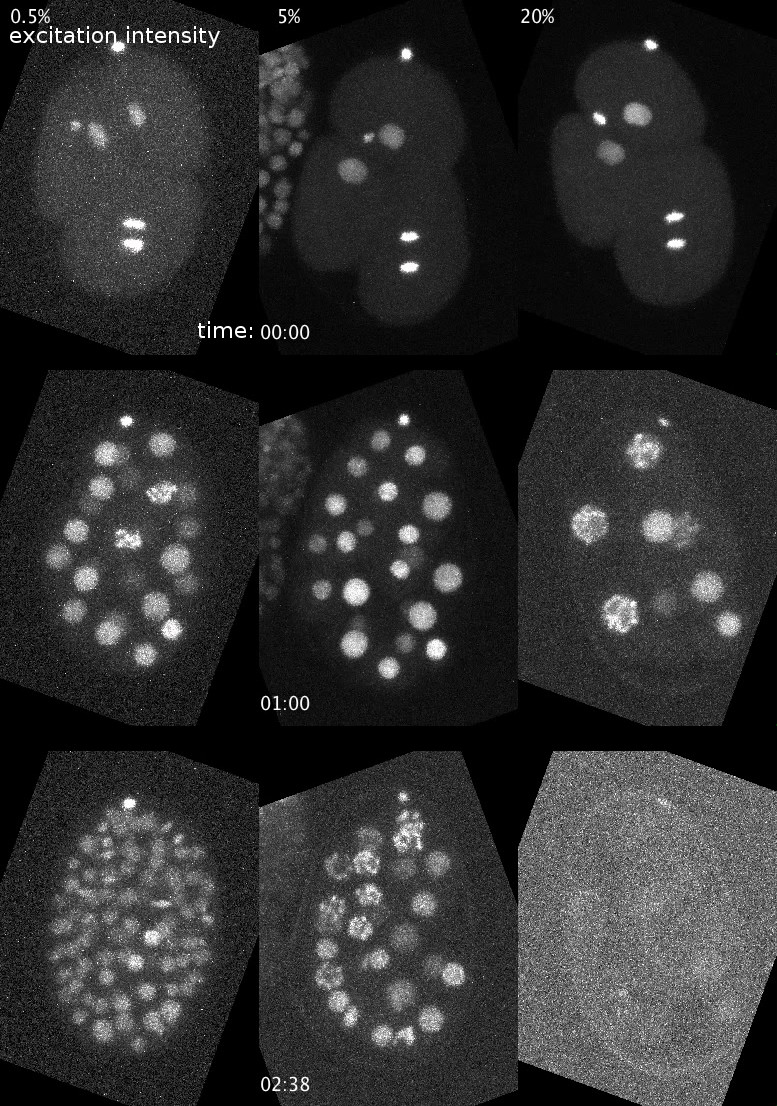
\includegraphics[width=12cm]{celegans-devel}
  \caption{Phototoxic effects while imaging the embryonal development
    of three \emph{C.~elegans} embryos (strain AZ212, histone-2B
    tagged with eGFP) with different excitation intensities. The
    embryo with lowest excitation dosage (left) develops fastest. The
    embryo with the highest dosage (right) ceases development and
    nearly all fluorophores are bleached after the experiment. Images by
    J.-Y. Tinevez (Institut Pasteur, Paris).}
  \label{fig:celegans-devel}
\end{figure}


In the rest of this chapter we give an overview of the photophysics of
fluorophores. We inicate why oxygen is such an important component in
the process of photobleaching and phototoxicity.  Then we give an
introduce conventional microscopes and finally we describe the noise
sources of CCD cameras.

